\newpage
\thispagestyle{sectioned}
\chapter{Arquitectura del Proyecto}

\section{Arquitectura de Wave}

	La arquitectura que soporta Wave tal y como la diseñó originalmente Google está estructurada en forma de capas que interactuan entre sí. De forma general y de abajo hacia arriba disponemos de las siguientes capas:
	
	\begin{itemize}
		\item Capa de Conexión Cliente/Servidor: Se encarga de gestionar la conexión entre cliente y servidor mediante el protocolo XMPP.
		\item Capa de Control de OT: Se encarga de gestionar la consistencia en tiempo real de los datos mediante la utilización de Transformaciones Operacionales (OT).
		\item Capa de Modelo de Datos Wave: Se encarga de gestionar los datos a nivel de las Waves que forman parte de una Conversación.
		\item Capa de Modelo Conversacional: Se encarga de gestionar los datos a nivel de las Conversaciones, junto a los documentos que las componen y los usuarios participantes (Ver Sección \ref{sec:waveModel}). En el caso de SwellRT se extendió este modelo a otro más generalizado llamado Modelo de Contenidos (Ver Sección \ref{sec:swellRTModel}).
		\item Capa de Interfaz de Cliente: API con operaciones para que el cliente interactue con el Modelo Conversacional subyacente mediante eventos. En el caso de SwellRT se extendió este API para utilizar el Modelo de Contenidos de esta tecnología. 
	\end{itemize}
	
	\begin{figure}[H]
	  \centering
	    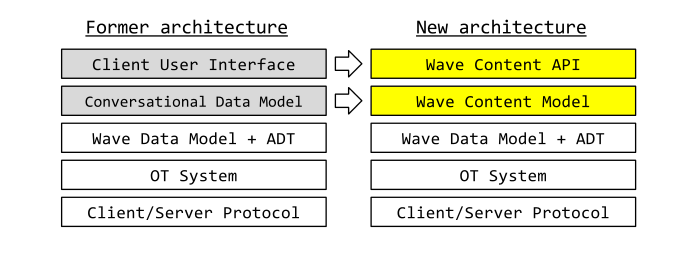
\includegraphics[keepaspectratio, scale=0.6]{Media/Captures/waveArch.png}
	  \caption{Arquitectura de Wave}
	  \label{fig:waveArch}
	\end{figure}
	

    \subsection{Modelo Conversacional Wave}\label{ssec:waveModel}
    
    Además de definir el protocolo del que hace uso Wave, Google definió un Modelo de Datos Conversacional \cite{ref:wave_conversation_model} que refleja la arquitectura de los datos que componen las conversaciones en Wave. Así, a grandes rasgos, podemos ver dichas conversaciones como documentos XML sobre los que los usuarios participantes (cualquiera es libre de unirse a una conversación en cualquier momento) actúan creando nuevos elementos o modificando los ya existentes. Este modelo de datos define una nomenclatura propia para los elementos que componen esta tecnología \cite{ref:wave_api_overview} \cite{ref:wave_white_paper}:
    
      \begin{itemize}
	\item \textbf{Wave}: Conjunto de wavelets (conversaciones).
	\item \textbf{Wavelet}: conjunto de documentos de una conversación y sus participantes.
	\item \textbf{Blip}: documento con el contenido de un mensaje en la conversación. Un blip puede tener otros blips dentro de él y los blips pueden ser publicados o no en función de si su visibilidad se extiende o no al resto de participantes de la conversación respectivamente.
	\item \textbf{Manifiesto conversacional}: documento con metadatos que definen la estructura de una conversación. 
	\item \textbf{Hilo conversacional}: conjunto de Blips consecutivos que forman parte de una conversación.
	\item \textbf{Extensiones} \cite{ref:wave_extensions}: pequeñas aplicaciones que se ejecutan dentro de una Wave y aportan nuevas funcionalidades que no forman parte del modelo conversacional básico. Pueden ser de dos tipos:
	  \begin{itemize}
	    \item \textbf{Gadget}: aplicación que se ejecuta en el contexto de una Wave y en la que todos sus usuarios participan.
	    \item \textbf{Robot}: aplicación que participa en una Wave a modo de usuario automatizado e interactúa con el contenido pudiendo modificarlo y responder a eventos por acciones de otros usuarios reales.
	  \end{itemize}
      \end{itemize}
      
    \begin{figure}[H]
	  \centering
	    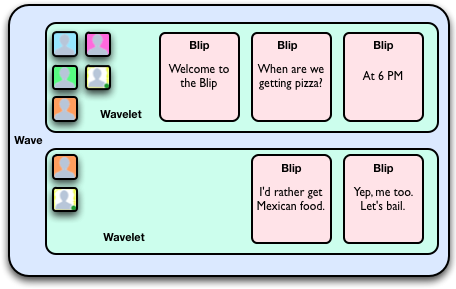
\includegraphics[keepaspectratio, scale=0.7]{Media/Captures/waveEntities.png}
	  \caption{Modelo Conversacional de Wave}
	  \label{fig:wave_model}
	\end{figure}
	
	\subsection{Modelo de Contenidos SwellRT}\label{ssec:swellRTModel}
	
	SwellRT \cite{ref:swellRT_github} (Swell Real Time) es un framework de desarrollo para Wave que forma parte del proyecto europeo P2P Value \cite{ref:p2pvalue}. Está basado en el servidor Wave In A Box \cite{ref:wave_in_a_box} (WIAB) y extiende sus funcionalidades cambiando el Modelo Conversacional original creado por Google por uno nuevo de propósito más general llamado Modelo de Contenidos. En este modelo nuevo podemos intercambiar estructuras de datos de forma colaborativa, federada y en tiempo real que combinen los siguientes 4 tipos: \textbf{Mapas, Listas, Strings y Documentos de Texto.}
	
	De esta manera la estructura de datos intercambiada constará siempre de un Mapa inicial (llamado ''root'') del cual colgarán a modo de árbol el resto de estructuras (de cualquiera de los cuatro tipos que maneja SwellRT) cuyos datos se gestionarán en tiempo real. Para ello existe también una API nueva que se encarga de la gestión de dicho arbol mediante la utilización de eventos que notifican de cambios en las estructuras de datos. Este modelo será el que utilicemos para la aplicación Android. El siguiente es un esquema de los cambios en el modelo original introducidos por SwellRT:
	
	
	\begin{figure}[H]
	  \centering
	    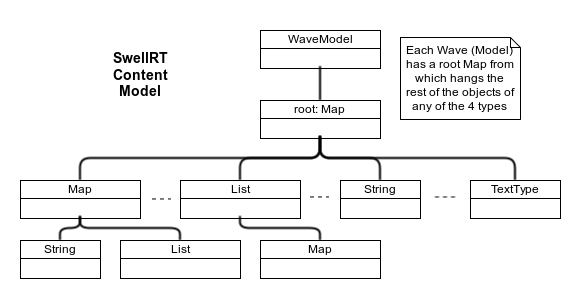
\includegraphics[keepaspectratio, scale=0.6]{Media/Captures/waveDataModel.png}
	  \caption{Cambio de Modelo de Wave}
	  \label{fig:wave_swellRT}
	\end{figure}

\section{Arquitectura de la aplicación}

La arquitectura de DemoCritics está compuesta por cuatro módulos principales de los que hablaremos en profundidad en las siguientes subsecciones. Como \textbf{Cliente móvil} tendremos la aplicación desarrollada en Android, que realizará peticiones HTTP al servicio web alojado en OpenShift \cite{ref:OpenShift}, una plataforma que permite alojar servicios web de forma gratuita. Dentro del servicio contaremos con un \textbf{Service RESTful} que será quien gestione las peticiones de la aplicación móvil mediante el protocolo HTTP. La \textbf{Base de Datos MySQL} alojada también en el servidor de OpenShift almacenará toda la información relacionada con la aplicación. La API del Service RESTful será quien actúe de intermediario entre las peticiones de la aplicación y las operaciones en Base de Datos.

\begin{figure}[H]
\centering
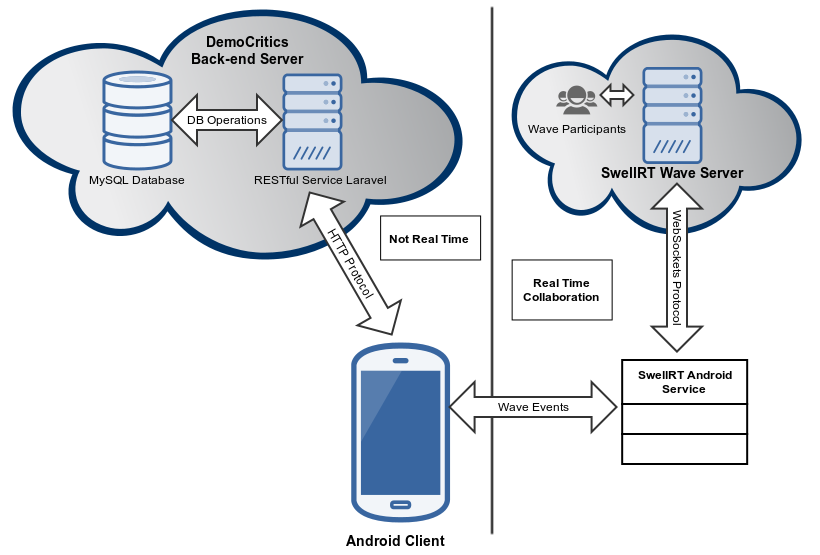
\includegraphics[keepaspectratio, scale=0.45]{Media/Diagrams/generalArchitectureDiagram.png}
\caption{Arquitectura general de la aplicación.}
\label{fig:architecture}
\end{figure}

Por otro lado, la aplicación hará uso del \textbf{Servicio Android} desarrollado en SwellRT-Android \cite{ref:swellRT_android_github} para conectarse con el servidor Wave alojado en \url{https://wave.p2pvalue.eu/} e intercambiar los datos que sea necesario mantener en tiempo real, es decir, la edición de una Propuesta de forma colaborativa entre varias personas.


\subsection{Base de datos}

En la implementación de la Base de Datos se ha utilizado un Modelo Relacional para la definición de las tablas. Utilizando MySQL \cite{ref:mysql} como sistema de gestión de base de datos (SGBD) y phpMyAdmin \cite{ref:phpMyAdmin} como herramienta de gestión gráfica de la base de datos.

La base de datos está formada por un total de nueve tablas donde se almacena toda la información relacionada con los programas de los partidos políticos, las propuestas ciudadanas, etc. y otros datos más técnicos como la gestión de los usuarios, la relación de los comentarios o la relación entre las secciones y comparativas entre otros.

\begin{figure}[!]
\centering
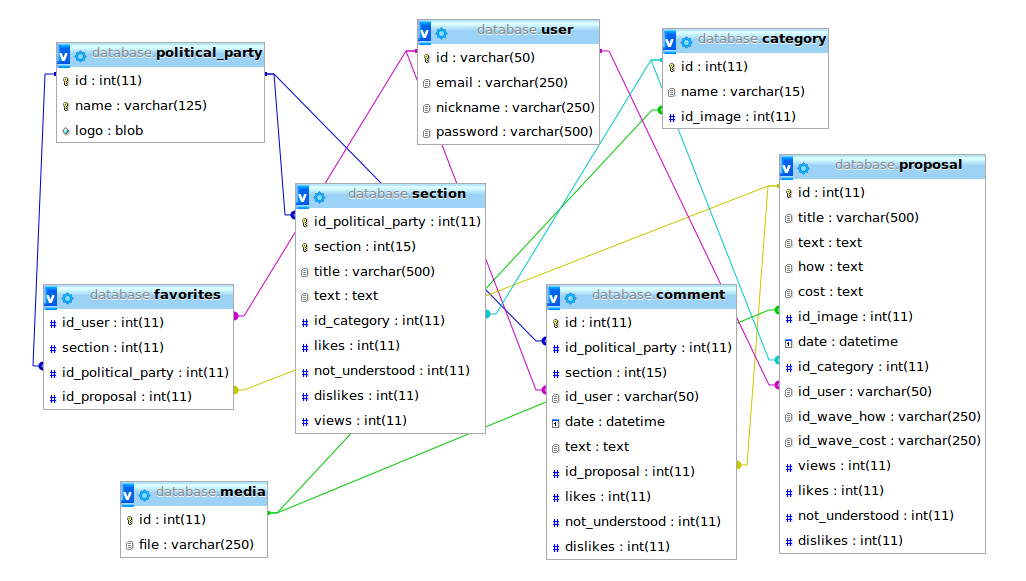
\includegraphics[keepaspectratio, scale=0.40]{Media/Captures/database.png}
\caption{Modelo entidad-relación de la base de datos.}
\label{fig:ermodel}
\end{figure}

Las tablas \textit{section} y \textit{political\_party} se utilizan para guardar información estática en la aplicación. Es decir, en la tabla \textit{political\_party} se almacenan los partidos políticos que se presentan a unas elecciones, y en la tabla \textit{section}, las diferentes secciones de un programa electoral. Tan sólo modificaremos las columnas de \textit{likes}, \textit{dislikes}, \textit{not\_understood} y \textit{views} para obtener estadísticas de uso de cada sección. El resto de las columnas permanecerán intactas (salvo que la redacción del programa cambie).

Definimos como datos \textit{estáticos} aquellos datos que permanecen intactos en la aplicación desde el inicio. Son datos que no requieren ser modificados y siempre permanecen tal y como estan, a no ser que surgiera algún fallo o imprevisto en la aplicación. Estos datos principalmente estarán formados por la información de los partidos políticos y sus programas. Entendemos que de cara a unas elecciones los partidos políticos no suelen cambiar su nombre, logo o lo que es el programa electoral. Por lo tanto esos datos permanecerán intactos durante el uso de la aplicación. Sin embargo, la aplicación contará con datos \textit{dinámicos} como aquellos datos que se irán generando y que con el tiempo pueden cambiar o eliminarse. Este tipo de dato estará relacionado con la mayor parte de la actividad del usuario con la aplicación. Por ejemplo, cuando un usuario agrega una nueva propuesta, esta propuesta será añadida como una fila más de la tabla \textit{proposals}. Además esta nueva fila estará sujeta a cambios que definirán su valoración, el número de comentarios, el número de visualizaciones, etcétera.

A continuación se procederá a explicar las tablas más relevantes de la base de datos:

\subsubsection{\textit{political\_party}}

Esta tabla contiene la información relacionada con los partidos políticos que se presentarán a las elecciones. Por tanto nos interesará guardar el nombre del partido, un logo que los identifique en formato \textit{blob} y un identificador único para relacionarlos con sus programas políticos.

\subsubsection{\textit{section}}

Esta es una de las tablas más complejas de la aplicación, pues contiene toda la información de los programas políticos. Encontraremos una clave primaria compuesta definida como \textit{id\_political\_party} y \textit{section}, que harán referencia a una sección concreta de un partido político. De esta forma nunca encontraremos una fila que contenga la misma sección de un programa del mismo partido político dos veces, ya que a cada sección le correspondería un solo partido político (para más información sobre la estructura del campo \textit{section} consultar el capítulo \ref{sssec:politicalProgramArch}). Por otro lado tenemos el contenido de la propia sección como del programa político, es decir, el título de la sección, el contenido en texto, etc. como datos \textit{estáticos} de la tabla. Y por último, los indicadores sociales de \textit{likes}, \textit{not\_understood}, \textit{dislikes} y \textit{views} como datos \textit{dinámicos} que se irán actualizando con la actividad de los usuarios.

\subsubsection{\textit{proposal}}

La tabla encargada de almacenar las propuestas que se van agregando a la aplicación. Estará definida por campos como un identificador único para la propuesta, el identificador del usuario que ha publicado la propuesta y el contenido de dicha propuesta. Estos datos serán \textit{estáticos} una vez que se inserten en la base de datos. Al igual que la tabla \textit{section}, también tendrá columnas son datos de carácter social y estadístico que irán modificándose con la actividad de los usuarios en el sistema. Por último, para diferenciar una propuesta publicada de una propuesta colaborativa, siendo esta última la que hace uso de \textit{SwellRT} para edición colaborativa, definiremos dos identificadores que harán referencia a los identificadores Wave de dos documentos colaborativos alojados en el servidor. De esta forma podemos saber cuando una propuesta se está desarrollando o está definitivamente publicada. Ya que para las propuestas publicadas en la aplicación, estas dos columnas tendrán el valor \textit{null}, ya que no harán referencia a ningún documento colaborativo.

\subsubsection{\textit{comment}}

Para almacenar los comentarios generados por los usuarios en la aplicación, se utilizará la tabla \textit{comment} que guardará el identificador del usuario y el texto del comentario. Esta tabla guardará los comentarios realizados en las secciones, como también los comentarios en las propuestas. De tal forma que un comentario para una sección de un programa político, irá acompañado de las columnas \textit{id\_political\_party} y \textit{section} de la misma manera que se relacionan las secciones de programas con partidos políticos. De lo contrario, si un comentario pertenece a una propuesta, deberá contener el identificador único de la misma mientras que los anteriores campos estarán a \textit{null}. El resto de las columnas estarán formadadas por datos de valoración y carácter social.

\subsubsection{\textit{opinion}}

Esta tabla será la referencia que almacenará las opiniones o valoraciones de un usuario en las propuestas y secciones de programas de la aplicación. De tal forma que se guardará el identificador del usuario que ha añadido esa opinión, acompañado del identficador de la propuesta si es el caso o el identificador de la sección del programa y el partido político en el caso de que se encuentre valorando una sección. Para indicar el valor de la opinión del usuario, es decir si ha valorado la sección o propuesta como \textit{like}, \textit{dislike}, etc, se utilizarán columnas que contendrán un entero que indicará el tipo de valoración que ha pulsado el usuario. De tal forma que el usuario siempre pueda cambiar su opinión o borrarla.

\subsection{Service REST} \label{ssec:seviceREST}

Para establecer la conexión de la aplicación desarrollada en Android con la Base de Datos hemos utilizado \textbf{Laravel} como \textit{framework} para desarrollo de servicios Web. Laravel \cite{ref:laravel} es un framework de código abierto para desarrollar aplicaciones web con PHP 5. Laravel permite además desarrollar una API REST (Representational State Transfer), un estilo de arquitectura software para sistemas hipermedia. Este término se originó en una tesis doctoral sobre la web escrita por Roy Fielding \cite{ref:RESTPhd}. La elección de Laravel como framework PHP se debió a su flexibilidad, la facilidad para programar la aplicación y el gran soporte que tiene de la comunidad. Además Laravel cuenta con una licencia de software libre MIT, lo que nos permite continuar utilizando software open-source en todo el proyecto. Es uno de los frameworks más populares actualmente.

\begin{figure}[H]
\centering
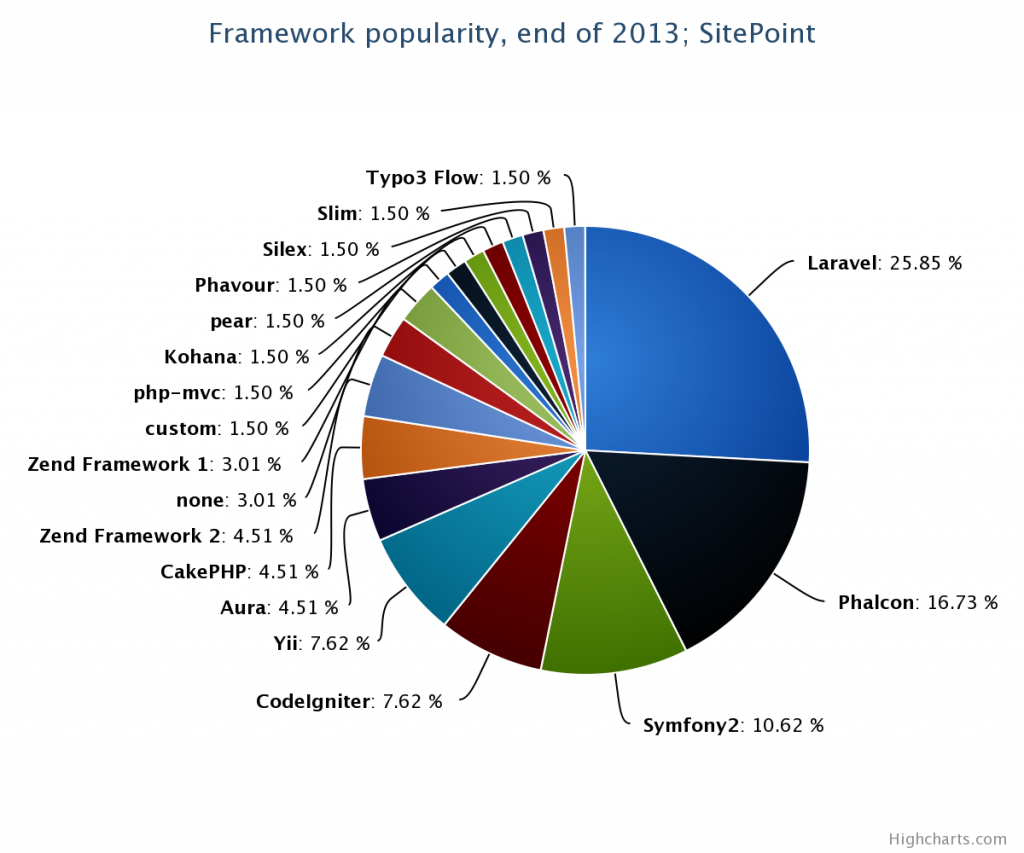
\includegraphics[keepaspectratio, scale=0.30]{Media/Captures/frameworkPopularity.png}
\caption{Frameworks PHP más populares. Fuente: SitePoint}
\label{fig:laravel5popularity}
\end{figure}

Laravel nos permite implementar un sistema RESTful para que el cliente móvil pueda hacer peticiones al servicio web y que dicho servicio responda a éstas de la forma que queramos. Estas peticiones se realizan mediante el protocolo HTTP. En función de la operación que deseemos hacer, clasificaremos estas funciones en el acrónimo \textbf{CRUD} \cite{ref:CRUD} (del original en inglés: \textbf{C}reate, \textbf{R}ead, \textbf{U}pdate and \textbf{D}elete).

\begin{table}[H]
\begin{tabular}{|c|c|c|m{6.25cm}|}
\hline
{\bf Petición} & {\bf Operación} & {\bf SQL} & \multicolumn{1}{c|}{{\bf Utilidad}}              \\ \hline
GET            & Leer            & SELECT    & Obtener un recurso almacenado en el servidor.    \\ \hline
POST           & Crear           & INSERT    & Crear un nuevo recurso en el servidor.           \\ \hline
PUT            & Actualizar      & UPDATE    & Actualizar un recurso almacenado en el servidor. \\ \hline
DELETE         & Borrar          & DELETE    & Eliminar un recurso almacenado en el servidor.   \\ \hline
\end{tabular}
\caption{Funciones CRUD}
\label{fig:CRUDtable}
\end{table}

Dependiendo de las peticiones que realicemos al servicio mediante el protocolo HTTP, el servidor nos devolverá un código de estado para obtener \textit{feedback} de lo sucedido. Por tanto distinguiremos diferentes códigos de estado cuando queramos obtener un recurso, actualizar un recurso, crear uno nuevo o borrarlo. En la siguiente tabla se definen los códigos de estado que puede devolvernos el servidor en función de nuestras peticiones.

\begin{table}[H]
\begin{tabular}{|c|c|m{7.5cm}|}
\hline
{\bf Petición} & {\bf Status Code} & \multicolumn{1}{c|}{{\bf Descripción}}                         \\ \hline
GET            & 200 (OK)          & El recurso solicitado ha sido devuelto correctamente.          \\ \hline
GET            & 404 (Not Found)   & El recurso solicitado no ha sido encontrado.                   \\ \hline
POST           & 201 (Created)     & El nuevo recurso ha sido creado correctamente.                 \\ \hline
POST           & 404 (Not Found)   & No se ha especificado el nuevo recurso a crear.                \\ \hline
POST           & 409 (Conflict)    & No se ha podido crear el recurso porque ya existe.             \\ \hline
PUT            & 200 (OK)          & El recurso ha sido actualizado correctamente.                  \\ \hline
PUT            & 204 (No Content)  & No se ha especificado el recurso que pretende ser actualizado. \\ \hline
PUT            & 404 (Not Found)   & El recurso a actualizar no ha sido encontrado.                 \\ \hline
DELETE         & 200 (OK)          & El recurso solicitado ha sido borrado.                         \\ \hline
DELETE         & 404 (Not Found)   & El recurso solicitado para borrar, no ha sido encontrado.      \\ \hline
\end{tabular}
\caption{Códigos de estado de la respuesta del servidor}
\label{fig:codeStateRestTable}
\end{table}

Usar un servicio RESTful nos proporciona una gran flexibilidad a la hora de independizar la tecnología del servidor de la del cliente. Mediante la arquitectura basada en peticiones HTTP no solo podremos hacer peticiones desde el cliente en Android, sino que más adelante podríamos desarrollar una versión web o incluso un cliente para iOS sin tener que modificar el servicio, ya que las peticiones HTTP serán las mismas.

\subsubsection{Arquitectura}

Laravel utiliza e implementa un funcionamiento basado en el patrón \textbf{MVC} (Model–View–Controller), separando el modelo de la vista, y delegando la gestión al controlador. En nuestro caso tendríamos un modelo almacenado en las tablas de la Base de Datos, donde se guardará toda la información dinámica y estática de la aplicación. El controlador sería en elcargado de gestionar las peticiones del cliente en Android en función del tipo de operación que requiera. Por último, tendríamos como vista el resultado devuelto por el servidor con los datos solicitados por el cliente, que a su vez los representaría en la aplicación móvil. Esta estructura de comportamiento hace independiente el modelo controlado por el servidor de la vista que obtiene el usuario final en su cliente móvil. Con esto conseguimos eleborar un código más claro y sencillo, así como también evitar conflictos entre el modelo y la vista.

\begin{figure}[H]
\centering
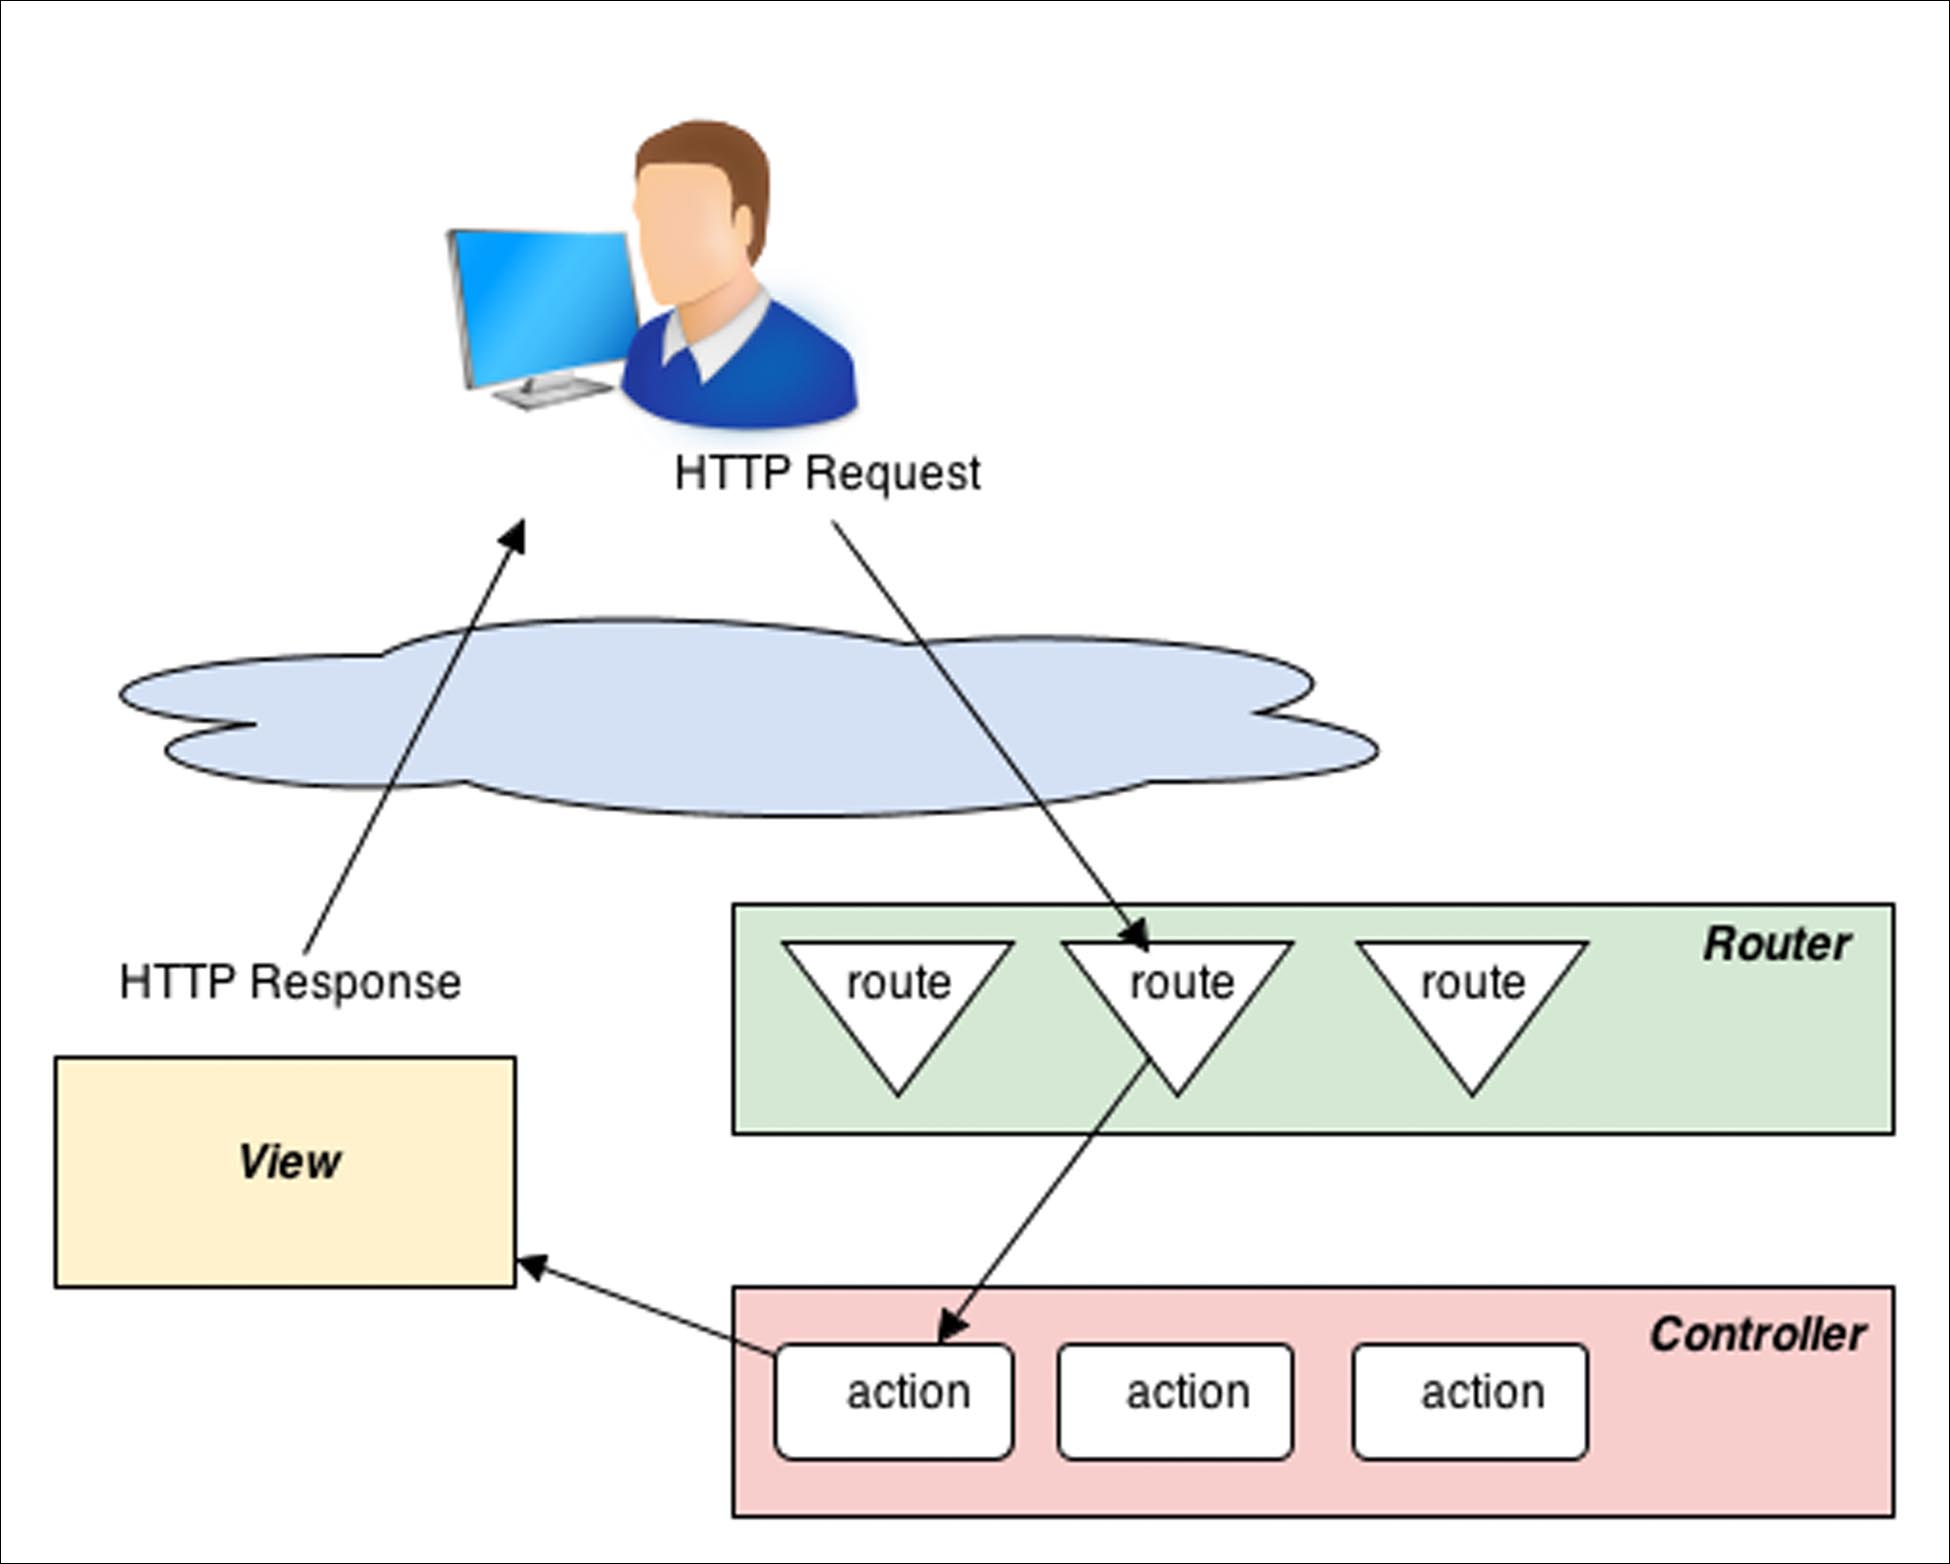
\includegraphics[keepaspectratio, scale=0.8]{Media/Captures/laravelArch.jpg}
\caption{Arquitectura de Laravel}
\label{fig:laravelArch}
\end{figure}

Para comprender la arquitectura de Laravel vamos a destacar tres componentes clave. En primer lugar tenemos una primera capa que gestiona las peticiones del cliente. Esta capa estará compuesta por una serie de \textbf{rutas} a las que el cliente realizará la petición en función de la operación que desee realizar. Después, en función de la ruta a la que haya realizado la petición, se adentrará en una nueva capa compuesta por \textbf{controladores} que se encargarán de procesar la petición y devolver al cliente lo que ha solicitado. El último componente será la \textbf{vista}, que puede ser representada de muchas formas. En nuestro caso, la vista estará compuesta por una serie de datos en formato JSON, que posteriormente el cliente móvil se encargará de representar en su propia vista. Teniendo en cuenta todo esto, procederemos a detallar un poco más estos tres componentes fundamentales.

\subsubsection{Rutas}

Cómo citábamos anteriormente, la primera capa de Laravel es un \textit{mapa de rutas} que definirá todos los caminos posibles para llegar a la funcionalidad requerida de los controladores. Todas las rutas estarán definidas en el fichero \textbf{routes.php}, alojado en la carpeta \textit{app/Http/routes.php} de nuestra instalación Laravel. El archivo \textit{routes.php} es un fichero muy simple escrito en PHP donde definiremos todas las rutas posibles. La definición de una ruta irá acompañada de tres valores. El primero de ellos será el tipo de petición que realizará el cliente (ver tabla \ref{fig:CRUDtable}), seguido de la definición de la URL por la que será accesible, y por último indicaremos el controlador responsable de procesar la petición. Aparte de indicar el controlador, también hay que indicar el método que procesará la petición dentro del controlador como veremos más adelante.

Para definir el conjunto de urls que forman el archivo \textit{routes.php}, hemos seguido una serie de buenas prácticas \cite{ref:practicesRESTful_API}, habituales a la hora de desarrollar una RESTful API. Normalmente utilizaremos nombres en lugar de verbos para acceder a los recursos. Por ejemplo, si queremos visualizar el listado de propuestas de la aplicación, utilizaremos la url \textit{/proposal}. Que será definida como:	

\lstset{
   language        = php}
\begin{lstlisting}[frame=single]	
Route::get('/proposal', 'ProposalController@index');
\end{lstlisting}

Así queda definida la ruta que accede a todo el listado de propuestas como una petición GET, que se encargará de procesar el controlador \textit{ProposalController} en su método \textit{index()}.

Para acceder a una propuesta en concreto, se pasará un \textit{id} para obtener el recurso adecuado. Este \textit{id} irá a continuación de la url anteriormente definida. Por ejemplo, si quisiéramos acceder a la propuesta cuyo id es igual a 5, definiríamos la siguiente ruta:

\lstset{
  language        = php}
  \begin{lstlisting}[frame=single]	
Route::get('/proposal/{id}', 'ProposalController@show');
\end{lstlisting}

Nótese que la ruta es la misma que la anterior, a la que hemos añadido un nuevo parámetro que deberá especificar el usuario. Así, la petición \textit{GET /proposal/5}, nos devolvería la propuesta con id 5. Si nos fijamos, el controlador también es el mismo, pero esta vez el método encargado de procesar la petición será \textit{show()}. Además, este método recibirá el parámetro \textit{{id}} que envíe el usuario en la petición.

Para crear una nueva propuesta en la aplicación, deberemos realizar una petición POST. Nuestra ruta será exactamente igual que la primera, pero antes deberemos especificar que se trata de una ruta que atenderá a una petición POST:

\lstset{
  language        = php}
\begin{lstlisting}[frame=single]	
Route::post('/proposal', 'ProposalController@create');
\end{lstlisting}

Donde una vez más en controlador \textit{ProposalController} se encargará de procesar la petición en el método \textit{create}. Si nos fijamos en la primera ruta dónde obteníamos las propuestas (\textit{GET /proposal}, es exactamente igual que la que acabamos de definir. Sólo les diferencia el tipo de petición que está realizando el cliente. Para definir otros tipos de peticiones como PUT o DELETE, usaremos la misma metodología. Un ejemplo del resultado final de las peticiones que podrían realizarse a una propuesta se puede ver en la Sección \ref{ssec:codeRoutesSimple} del Apéndice.

Para organizar el código y poder visualizarlo de forma clara utilzaremos grupos de rutas. Esto nos resultará especialmente útil cuando tengamos varias operaciones que realizar dentro de una misma dirección, definiendo una nueva ruta cuya función será definida a continuación, incluyendo las rutas que vienen dentro del grupo. Si nos fijamos en el ejemplo anterior, podemos observar como todas las url comienzan con \textit{/proposal}. Por ello no es necesario definir en cada línea la ruta \textit{/proposal}, si no que bastará con definirla en un único grupo que agrupará todas las rutas que comienzen de la misma forma. Así nuestro ejemplo anterior quedaría más claro y ordenado (ver Sección \ref{ssec:codeRoutesGroupe} del Apéndice).

De esta forma podemos visualizar todas las posibilidades agrupadas dentro de la dirección \textit{proposal}. Lo que nos permitirá utilizar grupos para ordenar funciones comunes dentro de un mismo prefijo, y además crear subgrupos dentro de los anteriores si tenemos algún prefijo repetido varias veces. Esto podría aplicarse a nuestro ejemplo anterior, agrupando las peticiones que requieren como parámetro un \textit{id} de la propuesta (ver Sección \ref{ssec:codeRoutesGroupeProposals} del Apéndice).

\subsubsection{Controladores}

Los \textbf{controladores} son los encargados de procesar todas las operaciones que intervienen en el modelo, es decir, en la información almacenada en la base de datos. Un controlador es un fichero escrito en PHP que será almacenado en la ruta \textit{/app/Http/Controllers} de la aplicación. Este fichero estará formado por una métodos y atributos que serán llamados desde las rutas definidas en la aplicación. Cada controlador hereda de una clase abstracta llamada \textit{Controller}, que a su vez hereda de la clase abstracta \textit{BaseController}. La cual implementa la funcionalidad básica de los controladores.

\begin{figure}[H]
\centering
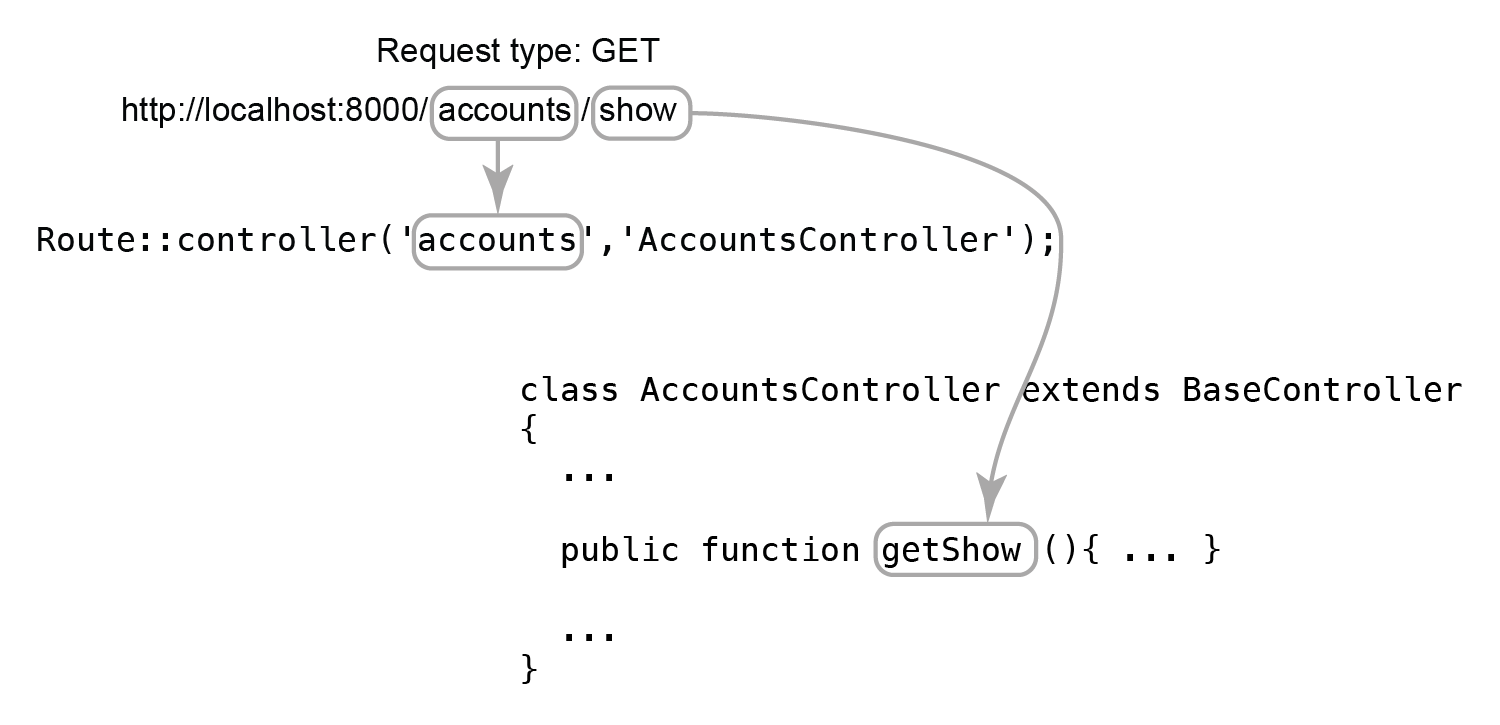
\includegraphics[keepaspectratio, scale=1]{Media/Captures/getDiagramMethod.png}
\caption{Camino desde la ruta al método del controlador.}
\label{fig:laravelArch}
\end{figure}

Dentro de un controlador definiremos aquellos métodos que correspondan con las rutas de la aplicación. Estos métodos procesarán la información del cliente, operando con los parámetros que haya obtenido, accediendo a la base de datos, y devolviendo una respuesta en función del éxito de la operación. Un ejemplo que muestra una implementación básica del método \textit{index()} del \textit{ProposalController}:se puede ver en la Sección \ref{ssec:codeControllerProposals} del Apéndice).

La conexión a la base de datos se encuentra configurada en el archivo \textit{/config/database.php}, por lo que la gestión de la conexión y desconexión será controlada por Laravel, lo que nos proporciona más independencia y versatilidad a la hora de programar. Como respuesta del método, Laravel utiliza por defecto un fichero JSON con los resultados de la variable a la que asignemos el resultado, o a la sentencia SQL de la consulta que estemos devolviendo. El siguiente ejemplo muestra cuál sería el resultado de realizar una petición GET a la dirección \textit{/proposal}:

\lstset{
  language        = c,    inputencoding=utf8}
\begin{lstlisting}[frame=single]
[
  {"id":1,"title":"Reducir la contaminaci\u00f3n en Madrid","text":"Actualmente la contaminaci\u00f3n en Madrid est\u00e1 llegando a unos l\u00edmites por encima de la media de las principales ciudades de la Uni\u00f3n Europea. Por ello deber\u00edamos reducir esa contaminaci\u00f3n ambiental acerc\u00e1ndonos a la media europea.","how":"Cerrando el tr\u00e1fico en determinadas zonas de Madrid. Distrito: Zona Centro.","cost":"Hacer 7 km de calles peatonales: 750.000 \u20ac","id_image":4,"date":"2015-05-06 00:00:00","id_category":4,"id_user":"6d823fa54c6d1a12","views":4,"likes":3,"not_understood":0,"dislikes":0}
]
\end{lstlisting}

\subsection{Cliente Android}

	La plataforma Android divide el desarrollo de una aplicación en dos partes: la implementación de la lógica detras de la aplicación mediante el uso de Activities \cite{ref:android_activities} o Services \cite{ref:android_service}, y la configuración del aspecto de la interfaz mediante Layouts XML \cite{ref:android_layout}. En las siguientes secciones hablaremos de algunos de los aspectos más destacados de este proyecto en referencia a dichas características de Android.

	\subsubsection{Interfaz Gráfica}
	
		En el desarrollo de esta aplicación quisimos utilizar un diseño plano basado en las últimas guias de diseño de Android disponibles en su última versión 5.0. Google denominó a este diseño plano ''Material Design''. 
	
		En Android, cuando creamos una Actividad (en su método ''onCreate()'') asignamos una Vista (''View'') a la actividad que representa la interfaz del usuario. Esta vista está definida en un archivo de Layout XML que deberemos modificar para crear la interfaz gráfica añadiendo componentes gráficos \cite{ref:android_widget} (''widgets'') y modificando sus atributos mediante etiquetas XML para adaptarlos a nuestras necesidades. Además podemos asignarles un identificador único para poder movernos por dichos widgets luego desde el código de la aplicación mediante una navegación en árbol utilizando el método ''findViewById()'' proporcionado por Android. 
		
		Estos componentes gráficos pueden ser los básicos proporcionados por Android (como cajas de texto, botones, listas, etc.) o se pueden crear \textit{Vistas Personalizadas} en caso de que los widgets básicos no aporten la funcionalidad deseada.
		
		En este último caso será necesario definir un Layout para la vista personalizada (que puede a su vez estar compuesto por widgets básicos o no) y una clase que posea referencias a los datos y a los componentes del layout que los albergarán.
		
		Sin embargo a menudo querremos usar varias de estas vistas, ya sean básicas o personalizadas, juntas dentro de una lista,  por lo que necesitaremos un \textit{Adaptador}\cite{ref:android_adapter} (''Adapter'') que haga de intermediario entre el layout y la clase que lo define para ''adaptar'' los datos que posee la clase a los componentes del layout que los muestran. 
		
		Veamos un ejemplo de esto con nuestra vista (widget) personalizada llamada \textbf{PartyWidget}, creada para mostrar cada uno de los elementos de la lista de Partidos Políticos que se visualiza en la aplicación. El funcionamiento de este widget personalizado esta formado por los siguientes tres elementos:
		
		\begin{itemize}
			\item \textbf{party\_widget.xml}: Layout XML que define la disposición de los dos componentes gráficos básicos que conforman esta vista: un ''ImageView'' para el logo del partido y un ''TextView'' para el nombre del partido.
			\item \textbf{PartyWidgetView.java}: Clase que define el objeto contiene referencias a los dos componentes anteriores (mediante sus IDs) y los datos de la imagen (de tipo Bitmap) y el nombre (String) del partido.
			\item \textbf{PartyWidgetAdapter.java}: Clase que extiende de un ''BaseAdapter'' de Android y define el adaptador que se encargará de gestionar una lista de elementos gráficos de un mismo tipo (en nuestro caso del tipo ''PoliticalParty'') y de crear las vistas que muestran los datos almacenados en dicha lista. El método más importante de un Adapter es el ''getView'', que crea la vista personalizada (en nuestro caso de tipo ''PartyWidgetView'') y le asigna los datos que hay dentro de cada elemento de la lista de la forma que nosotros le definamos. 
		\end{itemize}
		
		De esta manera, solo es necesario decirle al elemnto que contiene la lista de Partidos Políticos (en nuestro caso un ''GridView'' que permite visualizarlos en forma de rejilla que se adapta al tamaño de pantalla) que use como adaptador el PartyWidgetAdapter con los datos de la lista de Partidos Políticos que previamente nos hemos descargado. \\
		
				
		\underline{Navegación por Tabs}
		
		Tras la fase de investigación decidimos que sería interesante incluir en la aplicación distintos filtros para ver tanto las secciones como las propuestas más valoradas positivamente, más vistas, más comentadas, etc. Para implementar la vista de esta funcionalidad decidimos utilizar un diseño muy parecido al que utiliza Google en su tienda de aplicaciones Google Play para navegar de forma lateral mediante pestañas (''tabs'') deslizantes. En nuestro caso cada una de las tabs mostraría una lista (elemento ''ListView'' de Android) de elementos ordenados por distinto filtro.
		
		No obstante, el método utilizado por Google en anteriores versiones de Android basado en añadir Tabs a la barra superior (''Action Bar'')\cite{ref:android_actionBar} de la aplicación está actualmente obsoleto en el API 21, por lo que tuvimos que recurrir a la actual implementación de Google, que no se encuentra todavía dentro del API 21 de desarrollo. Es por eso que hubo que utilizar un par de clases (''SlidingTabLayout'' y ''SlidingTabStrip'') que definen las tabs utilizadas por Google en el diseño con ''Material Design''. Estas clases fueron extraidas del GitHub\cite{ref:android_tabGoogle} de la app que Google mostró en su aplicación de prueba cuando presentó ''Material Design'' a finales de 2014. Este elemento trabaja definiendo el contenido de cada Tab mediante la utilización de Fragmentos\cite{ref:android_fragment} (''Fragment'') de Android, que representan una porción de lo que se muestra dentro de una Actividad.
		
		Sin embargo, la vista (Layout) de una Sección y de una Propuesta dentro de esta lista sería muy similar (con su foto, título e indicadores sociales de número de likes, vistas, etc.) por lo que ¿cómo hacer para utilizar la misma vista en dos objetos que son de tipos distintos? La solución que encontramos para utilizar el mismo elemento de visulización (definido en el layout llamado ''top\_ranking\_item'') en ambos casos fue utilizar una interfaz que implementarían tanto la clase  ''Section'' como la clase ''Proposal'': la interfaz ''TopItem''.
		
	\begin{figure}[H]
	  \centering
	    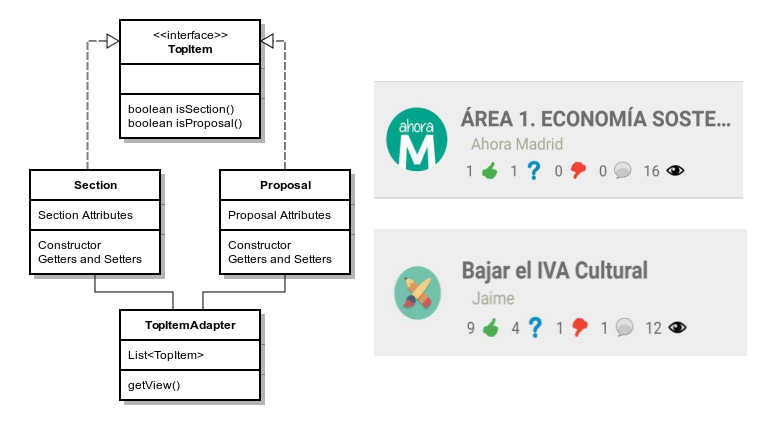
\includegraphics[keepaspectratio, scale=0.6]{Media/Diagrams/classDiagramTopItemAdapter.png}
	  \caption{Esquema de Implementación de TopItem (Con vista de Section y Proposal)}
	  \label{fig:topItemArch}
	\end{figure}
	
	De esta forma, las clases Section y Proposal implementan los métodos ''isSection()'' e ''isProposal()'' de la interfaz devolviendo true en cada caso respectivamente. Así, cuando dentro de nuestro Adaptador (''TopItemAdapter'') tratemos los elementos de su lista de TopItems en su método ''getView()'', podremos preguntar si se trata de un Section o un Proposal para rellenar la vista del ListView con los datos correspondientes a cada caso. Solo hace falta por tanto crear listas de Secciones o Propuestas y pasárselas al nuestro adaptador personalizado después de definirlo como adaptador para el ListView. \\
		
		\underline{Menús de Navegación}
		
		Con el objetivo de proporcionar al usuario una navegación por la aplicación que permita ir a cualquiera de sus secciones independientemente de en qué pantalla te encuentres actualmente, se decidió utilizar un menú lateral que se puede deslizar desde el lado izquierdo de la pantalla. Android permite añadir menús \cite{ref:android_menu} a las Actividades mediante métodos específicos de éstas, aunque en este caso son menús fotantes sencillos a los que se accede mediante el botón de opciones del móvil o de la app. 
		
		Nosotros queriamos utilizar el menú lateral deslizante presente en la mayoría de aplicaciones del estilo ''Material Design'' introducido por Google en su última versión de Android 5.0 (API 21), por lo que utilizamos un componente gŕafico llamado ''Navigation Drawer'' para ello. Este componente está presente en todos los layouts de la aplicación y contiene dentro un ''ListView'' con las entradas del menú. Cada una de estas entradas es asimismo un componente personalizado por nosotros, definido en el layout menu\_left\_item.xml (contiene un logo y el nombre de la entrada de menú). En consecuencia, y tal y como se ha hablado antes en esta sección, existirá también un Adapter ''MenuLeftListAdapter'' que se encargará de gestionar la vista de la lista de entradas del menú. Además, se le ha añadido una cabecera (''Header'') al menú, que contiene la información de nombre de Usuario y un botón para cambiar dicho nombre.
		
		Sin embargo, si todas las Actividades que componen la aplicación disponen de este menú, ¿Cómo hacer para evitar repetir el código de generación y configuración de dicho menú en todas las Actividades? La solución encontrada fue utilizar una Actividad padre llamada ''MenuActivity'' que se encargaría de generar y de albergar los métodos que configuran el menú. De esta manera, cualquier Actividad de la aplicación extendería de ''MenuActivity'' y llamaría a sus métodos de generación  coniguración de menú con una referencia a su propia vista de Layout (recordemos que cada Layout contiene el elemento ''Navigation Drawer'' necesario para mostrar el menú).
		
	\begin{figure}[H]
	  \centering
	    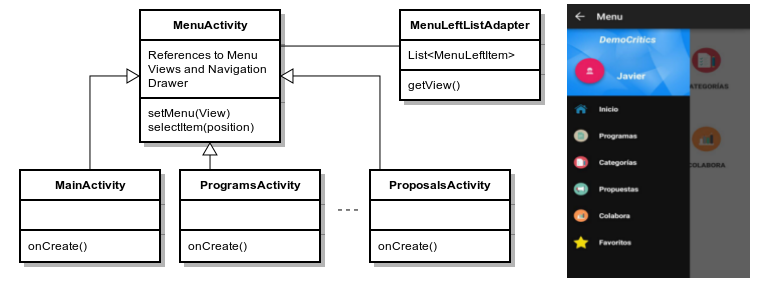
\includegraphics[keepaspectratio, scale=0.6]{Media/Diagrams/classMenuLeft.png}
	  \caption{Esquema de Implementación de Menú Izquierdo (Con vista del Menú)}
	  \label{fig:topItemArch}
	\end{figure}	
	
	Existe también en la aplicación un Menú derecho deslizable que muestra un Indice del Programa de un Partido Político para poder navegar por él de manera más sencilla (similar al que  utiliza la aplicación de la Wikipedia para navegar por un artículo). Este menú solo está presente en la actividad ''SectionViewerActivity'', ya que solo es necesario acceder al indice del programa cuando nos encontramos navegando por sus secciones. Utiliza también   para ello un ''Navigation Drawer'' similar al del otro menú antes explicado. No obstante, en este caso decidimos utilizar un tipo distinto de lista (''ExpandableListView'') que se diferencia de la lista normal en que posee dos niveles de navegación que se pueden expandir. De esta forma es necesario definir los layouts de los distintos niveles (''groups'') y los subniveles (''childrens'') dentro de cada uno. 
	
\begin{table}[H]
	\footnotesize
	\begin{center}
	\begin{tabular}{| c | c | c | m{4cm} |}
		\hline
		Adapter & Layout & Clase & Descripción \\ \hline
		PartyWidgetAdapter & party\_widget.xml & PartyWidgetView & Widget para mostrar un elemento de la lista de Partidos Políticos \\ \hline
		MenuLeftListAdapter & menu\_left\_item.xml & MenuLeftItem & Widget para mostrar las entradas del Menú lateral izquierdo. \\ \hline
		TopItemAdapter & top\_ranking\_item.xml & TopItem & Widget para mostrar un elemento de la lista con los Tops de Secciones y Propuestas. \\ \hline
		ListIndexAdapter & (solo muestra texto) & No es necesario & TextView (Android) que muestra los nombres del índice de un Programa Político. \\ \hline
		ExpandableListAdapter & \begin{tabular}[c]{@{}l@{}}list\_child\_item.xml\\ list\_group\_item.xml\end{tabular} & No es necesario & TextView que contienen los titulos de las distintas secciones y subsecciones (desplegables) del índice de un Programa Político. \\ \hline
		CommentListAdapter & comment\_item.xml & Comment & Widget para mostrar un comentario de un usuario dentro de la lista de comentarios de una Seccion o una Propuesta. \\ \hline
		SampleFragmentPagerAdapter & tab\_page\_*.xml & TabPageFragment & Widget para definir lo que contiene cada tab mediante Fragmentos cuya vista es generada de forma dinámica. \\ \hline
	\end{tabular}
	\end{center}
	\caption{Adapters, Views y Clases utilizadas en el proyecto}
	\label{fig:tableAdapters}
\end{table}
		
	\subsubsection{Estructuración de Programas Políticos}\label{sssec:politicalProgramArch}

		A la hora de almacenar los Programas Políticos en la Base de Datos tuvimos que estudiar la forma más adecuada de hacerlo para poder estructurar dichos programas en distintos niveles de secciones y subsecciones. En definitiva, el problema radicaba en cómo codificar la información de a qué nivel de anidamiento pertenecía cada Sección. Además, teniamos dos opciones: o bien el service REST devolvía un programa ya estructurado o la propia aplicación se encargaba de estructurarlos. \\
		
		\underline{Codificación en Base de Datos}
		
		En principio queríamos elegir una codificación que nos permitiera realizar una consulta a la base de Datos que devolviera las distintas secciones y subsecciones \textbf{en el orden en el que aparecen en el Programa}. Tras varios intentos con distintos campos de Strings y enteros como atributo de la tabla de Secciones en Base de Datos, decidimos que lo mejor sería utilizar un único número entero que codificara dicha información. Tras estudiar la composición de diversos programas identificamos que \textbf{no serían necesarios más de 4 niveles de anidamiento en subsecciones}. En consecuencia, el número estaría formado por 8 cifras, siendo cada dos cifras un nivel distinto de anidamiento. Veamos varios ejemplos de cómo funciona esta codificación:
		
	\begin{figure}[H]
	  \centering
	    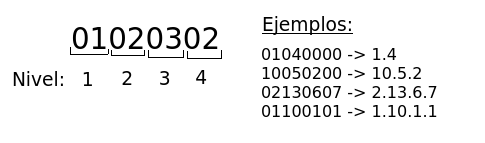
\includegraphics[keepaspectratio, scale=0.8]{Media/Captures/sectionsCodification.png}
	  \caption{Ejemplos de Codificación de Secciones y Subsecciones}
	  \label{fig:secCodification}
	\end{figure}	
	
	Utilizando esta codificación conseguimos que mediante una simple consulta SQL la Base de Datos nos devuelva todas las secciones del programa de un determinado partido de forma ordenada, siendo luego el Service REST el que pasará los resultados de esta consulta en JSON a la aplicación Android. \\ 
	
	\underline{Estructuración y Almacenamiento de Secciones}
	
	Con dicha codificación conseguiamos ordenar las secciones en el orden e el que aprecen en el programa, pero ahora debiamos guardarlas en la aplicación en unsa estructura que nos permitiera navegar por el programa de forma estructurada pudiendo en cada momento ver las subsecciones o volver a la seccion anterior. Decidimos por tanto \textbf{guardar el programa en una estructura en árbol formada por listas de listas}. De esta forma cada elemento de la lista sería un objeto del tipo Section que contendria la información de dicha seccion (titulo, texto, etc.) y otra lista con las subsecciones.
	
	Pero, ¿cómo construir esta estructura a partir de la lista ordenada que nos devuelve el Service REST? La solución encontrada fue utilizar una función que construyera dicho árbol de forma recursiva (Ver clase ''GetProgramsData.java'') sobre una Seccion ''root'' vacía que pertenecería a cada Partido Político. Dicha función recorrería la lista de secciones sin estructurar y para cada sección comprobraría su nivel de anidamiento para saber si colocarlo en el nivel actual, en el siguiente o en el anterior.
	
	Se puede ver el código de esta función de construcción del árbol en la Sección \ref{ssec:codeProgramTree} del Apéndice.
	  
	Además, como no queriamos tener que descargarnos el programa continuamente, esta estructura en forma de arbol se guardaría en una clase llamada ''PoliticalGroups'' que alamacenaría el listado de Partidos Politicos y para cada unode ellos almacenaría la estructura en árbol de su programa (su nodo ''root''). Esta clase implementa el \textbf{patrón de diseño Singleton} para asegurar que solo exista una instancia de ella, accesible desde cualquier punto de la aplicación. 
	  
	\begin{figure}[H]
	  \centering
	    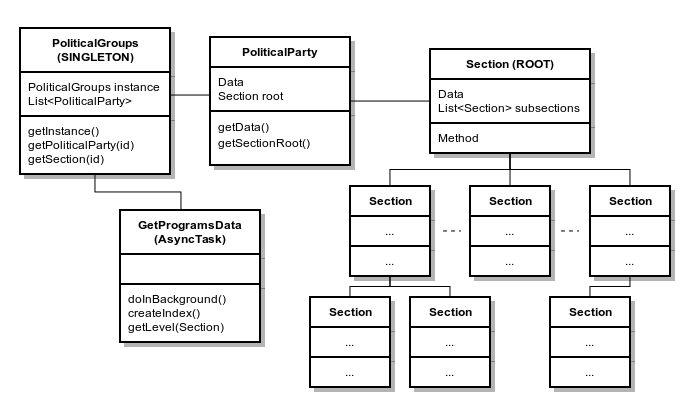
\includegraphics[keepaspectratio, scale=0.6]{Media/Diagrams/classSectionTree.png}
	  \caption{Esquema de estructura en árbol de Programa Político}
	  \label{fig:classSecTree}
	\end{figure}	
	
	\subsubsection{Conexión y Peticiones a Service REST y Base de Datos}

		Las peticiones de información a Base de Datos (ya sea para crear datos, descargarlos o modificarlos) se realizan mediante el protocolo HTTP enviando dichas peticiones al Service REST (Ver Sección \ref{ssec:seviceREST}). Para enviar dichas peticiones es necesario por tanto realizar una conexión HTTP al Service REST desde la aplicación Android. Aprovechando la experiencia previa adquirida durante la migración de Wave (Ver Sección \ref{sssec:conHttp}), decidimos utilizar la librería ''HttpURLConnection'' de Android y un esquema basado en AsyncTask que ejecutan el proceso de conexión y descarga de datos en un thread separado del UI Thread tal y como recomienda Google hacer para trabajar con conexiones de red\cite{ref:android_networking}.
		
		Así, en función de la operación que se quiera hacer en Base de Datos, para cada tipo de consulta existirá un AsyncTask encargado de conectarse al servidor con la URL apropiada y tratar los datos en JSON que este le pueda devolver, ya sea para mostrarlos o guardarlos en algún objeto de la aplicación. De forma general podemos identificar cuatro tipos de peticiones al servidor (Ver tabla \ref{fig:CRUDtable}).

Con el objetivo de no repetir código decidimos estructurar el esquema de peticiones HTTP mediante herencia de AsyncTasks. El siguiente diagrama esquematiza la estructura: 

	\begin{figure}[H]
	  \centering
	    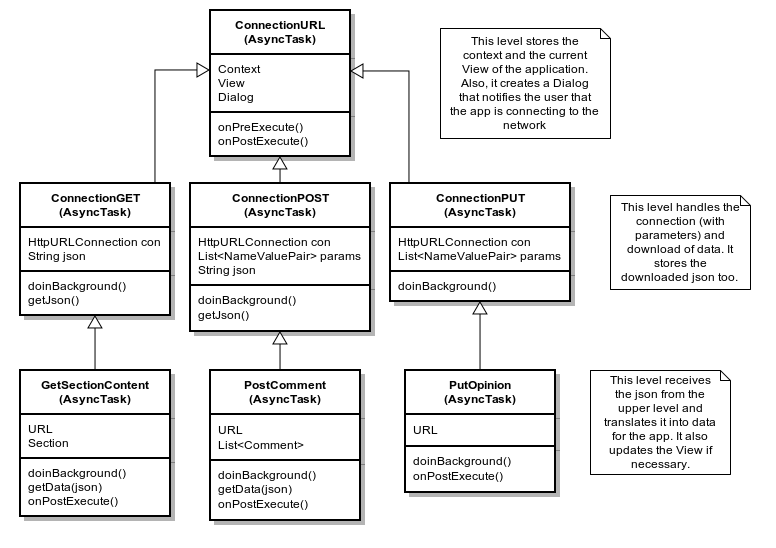
\includegraphics[keepaspectratio, scale=0.6]{Media/Diagrams/classDiagramAsyncTask.png}
	  \caption{Esquema de Clases de Conexión HTTP mediante AsyncTask}
	  \label{fig:classConnectionTree}
	\end{figure}	
	
	Hace falta también actualizar la vista del usuario cuando se reciban los datos. Como un AsyncTask se ejecuta en un hilo aparte diferente del UI Thread (para no bloquear la interacción con el usuario), a priori no tiene acceso a la vista (Layout) que se le está mostrando al usuario. Por esta razón la solución que encontramos fue guardar una referencia a la vista del usuario dentro del AsyncTask (ver clase ''URLConnection''). De esta manera en su método ''onPostExecute()'' que se ejecuta nada más terminar la operacion de conexión del ''doInbackground()'', obtenemos dicha vista y la actualizamos con los datos recién descargados. Este método de actualización de la vista es el que se utiliza en todos los casos. \\
		
		\underline{Comprobación de Conexión a Internet}
		
		Por otro lado, para llevar a cabo un control de errores en la conexión al Service REST, antes de ejecutar la tarea en el AsyncTask comprobamos el estado de la conexión del dispositivo móvil para asegurarnos de que el usuario dispone de conexión a Internet. En caso contrario se le muestra un mensaje de aviso para que compruebe sus conexiones y no se lleva a cabo la tarea de conexión en el AsyncTask. Aprovechando que todas las actividades extienden de ''MenuActivity'' dicho método de comprobación se encuentra dentro de esa clase. Además, fue necesario definir el siguiente permiso en el ''AndroidManifest.xml'' de la aplicación para acceder a la información de estado de la conexión del dispositivo:
		
		  \lstset{language=XML, breaklines=true, autogobble=true, basicstyle=\ttfamily\footnotesize}
	  \begin{lstlisting}[frame=single]
	  <uses-permission android:name="android.permission.ACCESS_NETWORK_STATE" />
	  \end{lstlisting}
		
	\subsubsection{Gestión de Usuarios: ID de Android} \label{sssec:idUser}
	
		Como esta versión de la aplicación no maneja información critica y sensible del usuario decidimos utilizar un método de autenticación basado en el ID almacenado en el dispositivo móvil. En Android existen varios identificadores (IMEI, ID de dispositivo, ID de Android..) teniendo cada uno de ellos características distintas. En nuestro caso \textbf{decidimos utilizar el ID de Android} \cite{ref:android_secure} ya que es único para cada instalación de sistema operativo y acceder a su valor no requiere de permisos especiales en la aplicación. Se trata de un número de 64 bits en formato hexadecimal al cual se accede directamente mediante la variable del sistema ''Secure.ANDROID\_ID''.
		
		El acceso a este identificador se produce nada más ejecutar la aplicación en su actividad ''MainActivity'' y se guarda de forma estática en la clase ''User'' para poder acceder a él desde cualquier punto de la aplicación. Con el identificador también se accede a la Base de Datos para descargar el nombre de Usuario que se corresponde con dicho identificador. Este nombre se muestra en el menú izquierdo de la aplicación y se puede cambiar desde ahí. De esta manera, todo el contenido generado por un usuario (Opiniones, comentarios, propuestas,...) se guarda tambien en base de datos asociado a este identificador único.
		
	\subsubsection{Servicio Android, Conexión con Wave/SwellRT y Gestión de Propuestas Colaborativas}

		Al servicio (ServiceSwellRT) desarrollado durante la migración de SwellRT a Android (Ver Sección \ref{ssec:migrationResult}) se le añadió encima el API del Modelo de Contenidos de SwellRT (Ver Sección \ref{ssec:swellRTModel}). Este API trabaja con Waves (o "modelos") con identificadores únicos, y dentro de cada modelo habrá un objeto "root" del tipo Mapa del que colgarán los distintos objetos con los que podremos jugar de cada uno de los cuatro tipos básicos de datos: Mapas, Listas, Strings y Documentos de Texto.
		
		En este proyecto utilizamos SwellRT para soportar la edición de propuestas colaborativas. Este tipo de propuestas puede tener asociadas dos textos colaborativos que se corresponden con la manera de llevar a cabo la propuesta y cómo financiarla. Para implementar esto con wave será necesario por tanto crear una wave por cada propuesta colaborativa, que tendrá asociados a su mapa 'root' dos objetos del tipo Documento de Texto (TextType). Este tipo permite crear documentos colaborativos que pueden ser editados en tiempo real por todo aquel usuario de wave que esté registrado como participante. 
		
		El funcionamiento del Servicio Android de conexión con SwellRT exige primero enlazar (''bind'') la Actividad actual con el Service para poder hacer uso del API. Después de enlazar, podremos registrarnos en el servidor SwellRT y crear, abrir, cerrar o borrar waves, a las que tambien podremos añadir participantes y nuevos objetos de los cuatro tipos antes mencionados. 
		
		En SwellRT se accede a estos objetos a partir del identificador que les otorguemos al crearlos, en este caso se creará dentro de cada wave dos TextTypes con identificadores "howProp" y "costProp" para cada uno de los textos colaborativoas antes mencionados. Asimismo, cada propuesta tendrá asociada una wave con un identificador único generado por el servidor al crearse la wave. Este identificador será el que guardemos en la base de datos para que cualquier usuario pueda acceder a la edición colaborativa de la propuesta. El siguiente es un esquema del uso de SwellRT en el proyecto.
		
	\begin{figure}[H]
	  \centering
	    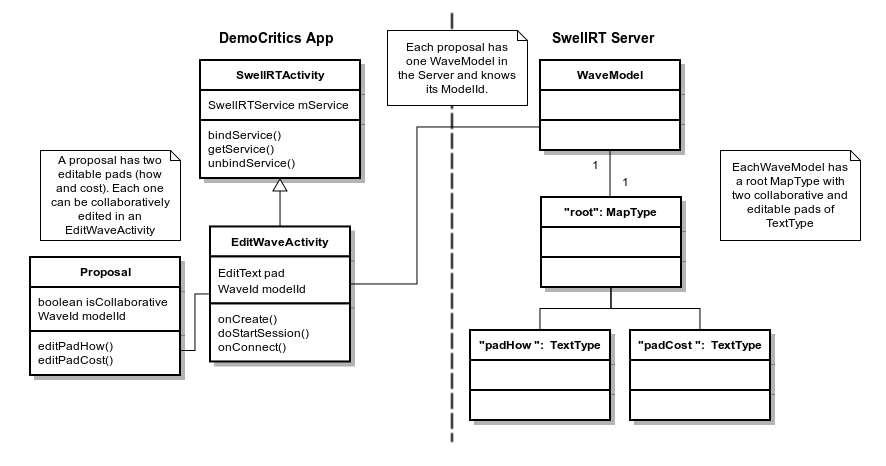
\includegraphics[keepaspectratio, scale=0.5]{Media/Diagrams/collaborativeProposalDiagram.png}
	  \caption{Esquema de Uso de Wave/SwellRT}
	  \label{fig:diagramUseSwellRT}
	\end{figure}	
			
		En el caso de DemoCritics lo primero que tendremos que hacer será registrar al usuario usando su ID (Ver Sección \ref{sssec:idUser}). Esto se hace en el ''MainActivity'' al ejecutar la aplicación.  Una vez registrado solo será necesario utilizar el ServiceSwellRT para llevar a cabo dos actividades: crear una nueva propuesta colaborativa y editar una propuesta ya creada. 
		
		Un ejemplo de cómo registrarse con SwellRT se puede encontrar en el Apéndice \ref{ssec:waveRegister}. \\

		\underline{Crear Propuesta Colaborativa}
		
		Esta es una opción que se le ofrece al usuario en el caso de que, al hacer una propuesta nueva, deje alguno de los campos de ''¿Cómo lo haría?'' o de ''¿Cómo lo financiaría?'' en blanco. En tal caso, lo primero que se hace es hacer un login en el servidor Wave llamando al método ''startSession'' del Service. Una vez que se ha iniciado sesión, se abre un nuevo modelo (wave) en el servidor para esta propuesta y se obtiene el Id (''WaveId'') de dicho modelo creado para guardarlo en la base de datos junto al resto de datos de la propuesta. Además, se le asocian al elemento ''root'' del modelo uno o dos documetnos colaborativos del tipo TextType llamados ''padHow'' y ''padCost'' en función de si ha dejado los dos campos vacíos o solo uno. Por último se añade como participante del modelo creado al usuario que lo ha creado (su ID\_USER). Cabe destacar que la mayor parte de la programación con el serviceSwellRT se lleva a cabo mediante callbacks que responden a eventos como iniciar sesión, crear modelos, etc.
		
		Un ejemplo simplificado del código encargado de crear el modelo se puede ver en el Apéndice \ref{ssec:waveCreateModel}.\\
		
		\underline{Editar Propuesta Colaborativa}

		Cuando un usuario quiere echar una mano a otro en la redacción de su propuesta, puede acceder a la propuesta colaborativa y editar los campos de ''¿Cómo lo haría?'' o de ''¿Cómo lo financiaría?'' en función de en qué necesite ayuda el usuario. Para cada uno de estos campos existe un ''pad'' en el servidor wave asociado a una wave cuyo identificador ''WaveId'' está guardado en la base de datos. Cuando el usuario pulsa en uno de los dos campos, se abre una nueva actividad ''EditWaveActivity'' que le ofrece un campo ''EditText'' de Android en el que puede escribir y ver lo que otros escriben en tiempo real. Para esto hace falta abrir una sesión en Wave, abrir el modelo con su WaveId, obtener el modelo y el pad, y asociar (''bind'') el pad a el EditText del usuario para que el servicio sea capaz de obtener los eventos de escritura del usuario.
		
		Un ejemplo simplificado del código encargado de abrir el modelo y asociar el pad colaborativo se puede ver en el Apéndice \ref{ssec:waveOpenPad}.
		
		

